%!TEX root = ../main/main.tex
\section{Component View} % (fold)
\label{sec:component_view}
This section highlights the main features and roles of every component of the system. Moreover it describes the internal interfaces between different classes of every component.\\
External interfaces between components are described in \emph{section \ref{sec:components_interfaces}}.
\subsection{\nameref{comp:server}} % (fold)
\label{sub:nameref_}
The \nameref{comp:server} is composed of:

\paragraph{Back-End Application} % (fold)
\label{par:back_end_application}\hfill \\
As stated in \emph{section 1.2.2} of the \emph{RASD}, the \emph{Back-End Application} is the system component that handles most of the business logic.\\
The application is written in \emph{Java EE} and to fulfill its tasks (see \emph{section 3.5.3} of the \emph{RASD}) it needs to interface with the Internet network using the \emph{HTTPS protocol} and the \emph{JAVA API for RESTful Web Service}\footnote{See \url{https://jax-rs-spec.java.net/}}, with a \emph{MySQL database} and with external Google Maps API.\\

\subparagraph{Back-End Internal Interfaces}
\label{subpar:back_end_interfaces}
The \emph{Back-End Application} is built to be very modular and to grant \emph{interchangeability} between components.\\
There are four main classes that constitute the kernel of the application :
\begin{itemize}
	\item \textbf{QueueManager} Handles queue policies. 
	\item \textbf{RideManager}  Creates and manage rides. Is connected to the \emph{RequestManager} via the \emph{RideManagerInterface} and directly depends on \emph{QueueManager}
	\item \textbf{ActorManager} Create and update data about users an taxi drivers. Is connected to the \emph{RequestManager} via the \emph{ActorManagerInterface}
	\item \textbf{PositionManager} Update taxi drivers position. Is connected to the \emph{RequestManager} via the \emph{PositionManagerInterface} and directly depends on \emph{QueueManager}
	\item \textbf{RequestManager}	Get and build \emph{Request} object from the requests received via \emph{HTTP}
\end{itemize}

\paragraph{MySQL Database} % (fold)
\label{par:mysql_database}\hfill \\
The MySQL database fulfills the task off storing and granting access to all the data generated and used by the service.\\
A \emph{database dump} is performed daily during the period of minor activity of the service \footnote{At first, when no activity data is available, the dump will be performed at 04:00 A.M}.\\
The connection between the \emph{Java EE} application and the databased is supported by the \emph{JDBC connector}\footnote{See \url{http://dev.mysql.com/downloads/connector/j/}}.\\


\subsection{User Client} % (fold)
\label{sub:user_client}
Different real clients are available to the end users of the system.\\
As stated in \emph{section 1.2.2} of the \emph{RASD} a native mobile application is developed for Android, iOS, Blackberry and WP.\\
Moreover a Web Application is also available.\\
To fulfill the requirements expressed in \emph{section 3.5.1} and \emph{section 3.5.2} of the \emph{RASD}, all the clients need to communicate with the \nameref{comp:server} making calls to the REST API using platform specific API for REST HTTP calls.

% subsection user_client (end)

\subsection{Taxi Driver Client} % (fold)
\label{sub:taxi_driver_client}
Different real clients are available to the taxi driver registered to \emph{myTaxiService}.\\
As stated in \emph{section 1.2.2} of the \emph{RASD} a native mobile application is developed for Android, iOS, Blackberry and WP.\\
To fulfill the requirements expressed in \emph{section 3.5.1} and \emph{section 3.5.2} of the \emph{RASD}, all the clients need to communicate with the \nameref{comp:server} making calls to the REST API using platform specific API for REST HTTP calls.
% subsection taxi_driver_client (end)
\subsection{Clients Internal Interfaces}
\label{sub:back_end_interfaces}
Mobile clients are composed mainly of subclass of platform specific components.\\
Interfaces between components are therefore specified in the SDK of each platform.
However it's important to highlight that every mobile application has to interface with a \emph{Network Component} that handles \emph{HTTP} requests.\\

\newpage
\vfill
\begin{figure}[h!t]
\caption{BackEnd Class Diagram}
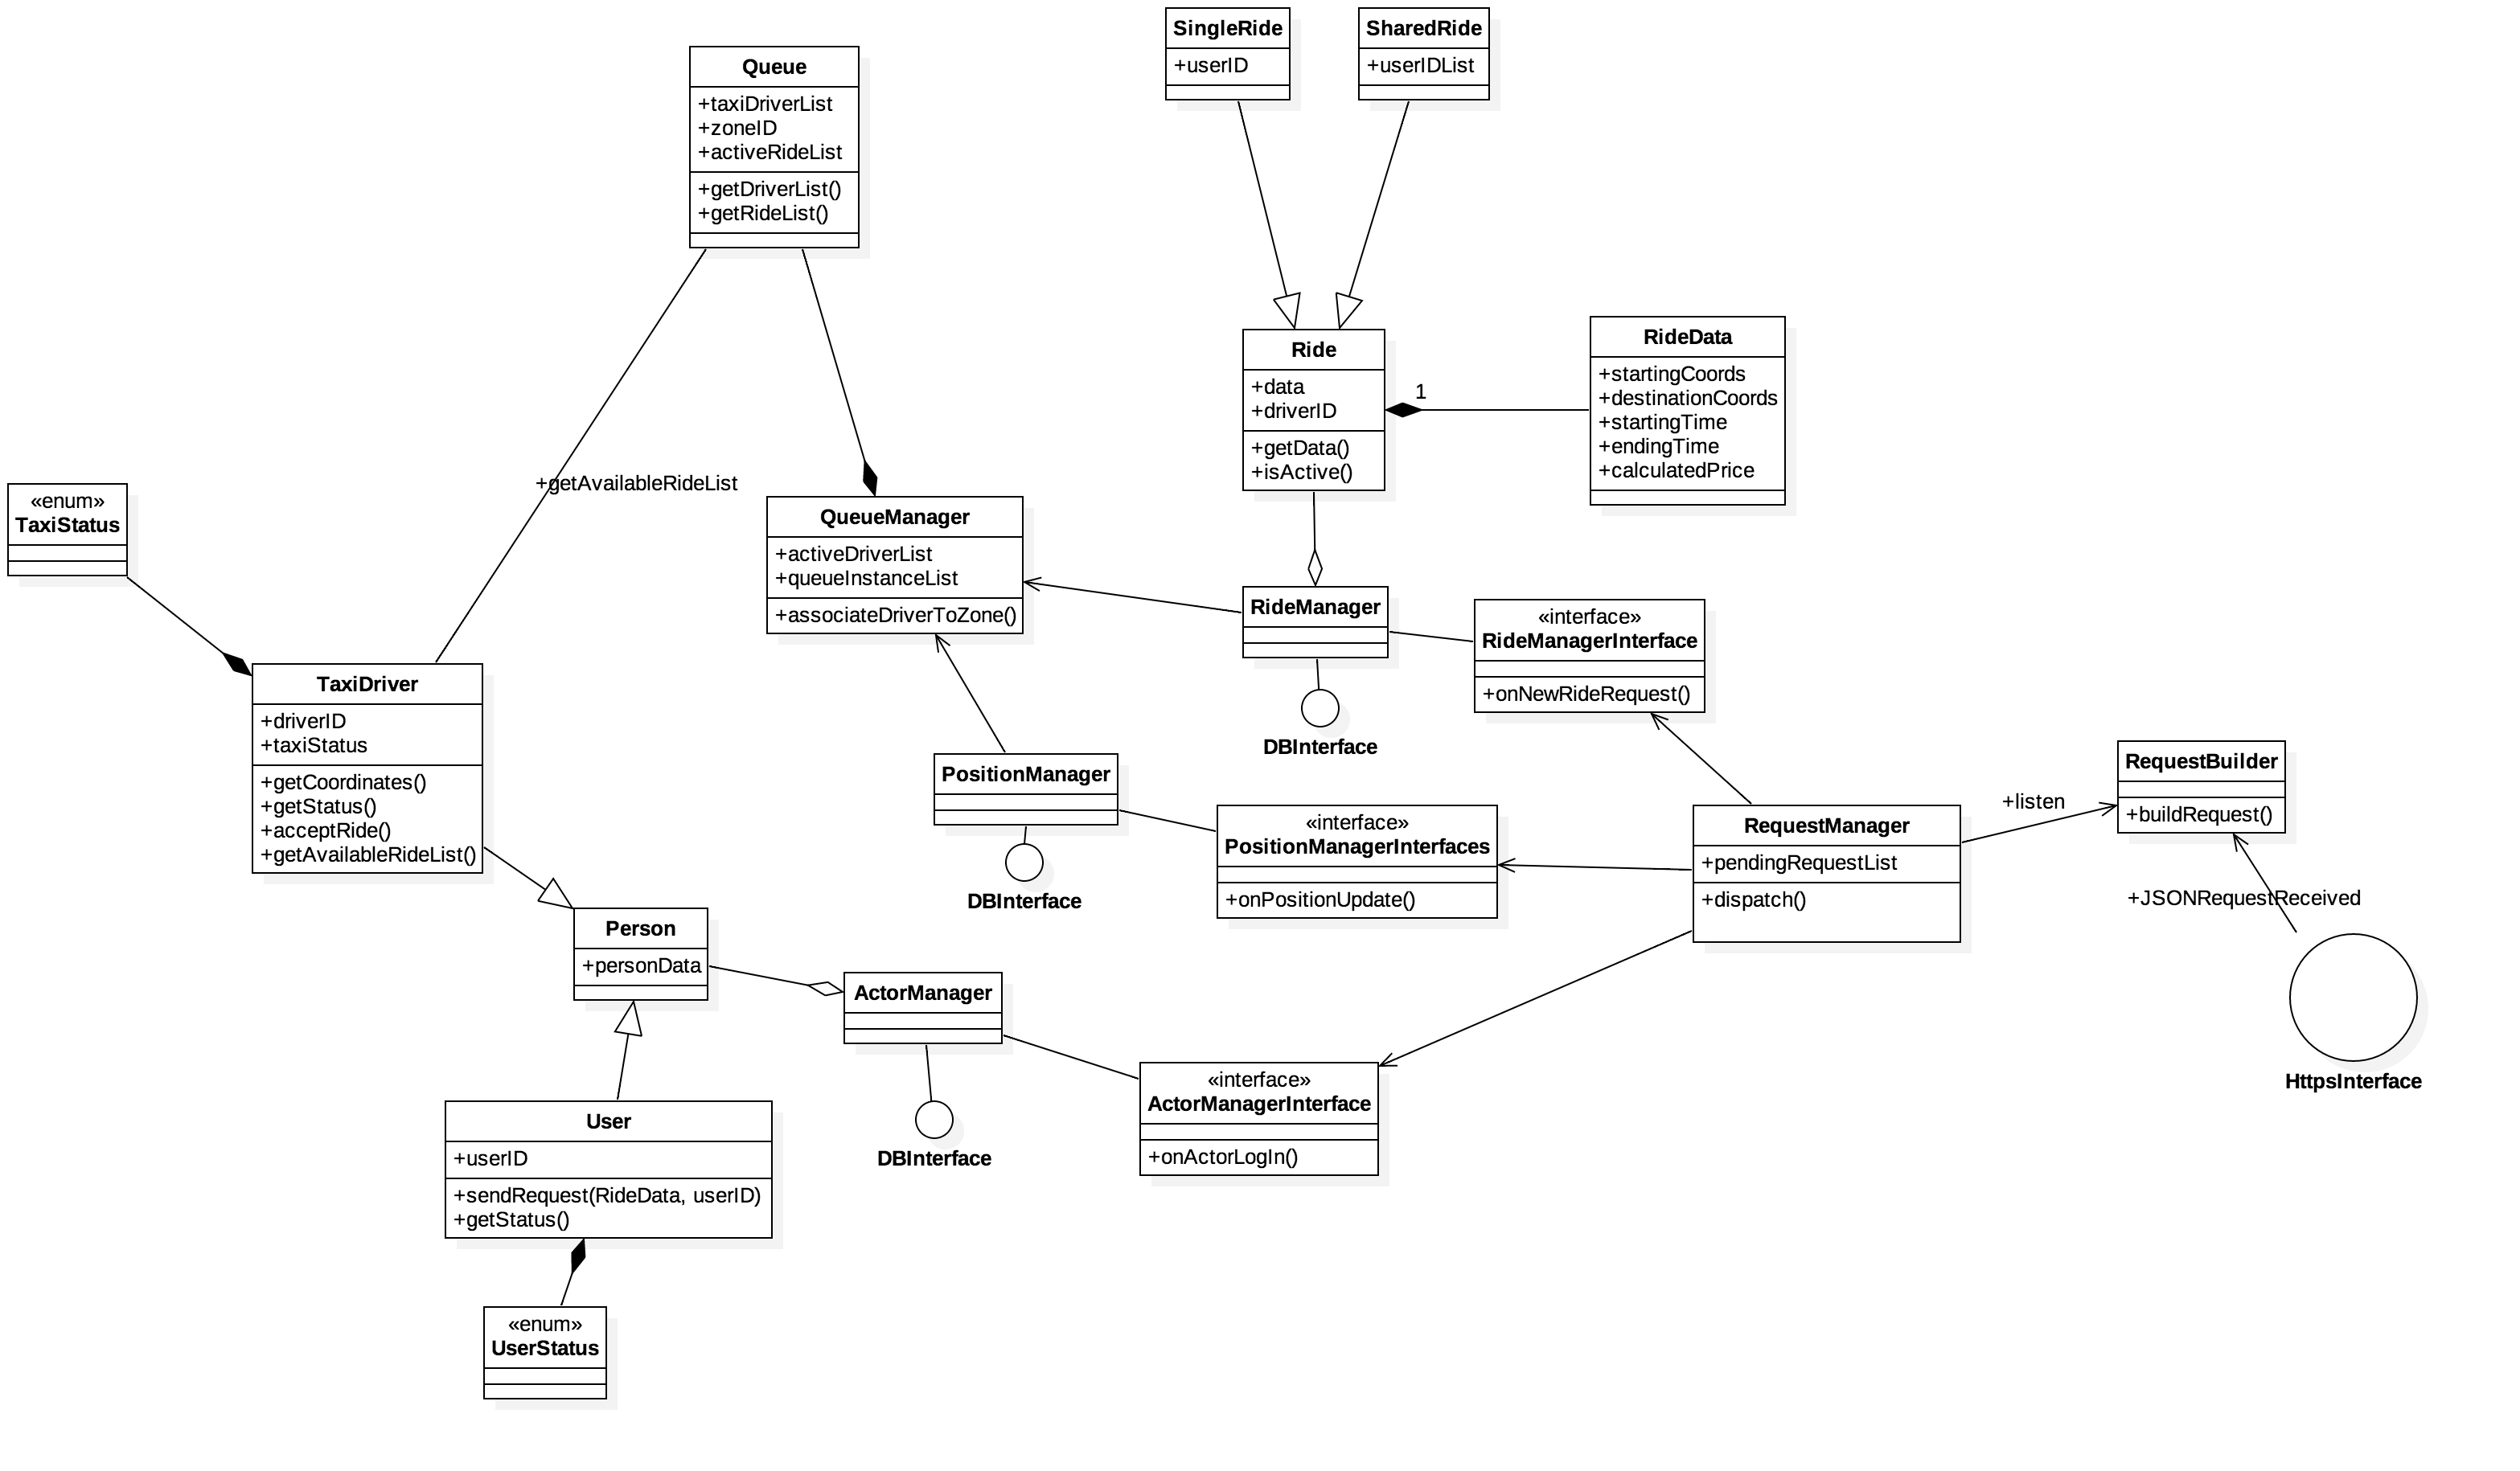
\includegraphics[width=\textwidth]{diagram/png/backendClass}
\centering
\end{figure}
\vfill
\clearpage

\newpage
\vfill
\begin{figure}[h!t]
\caption{User App Class Diagram}
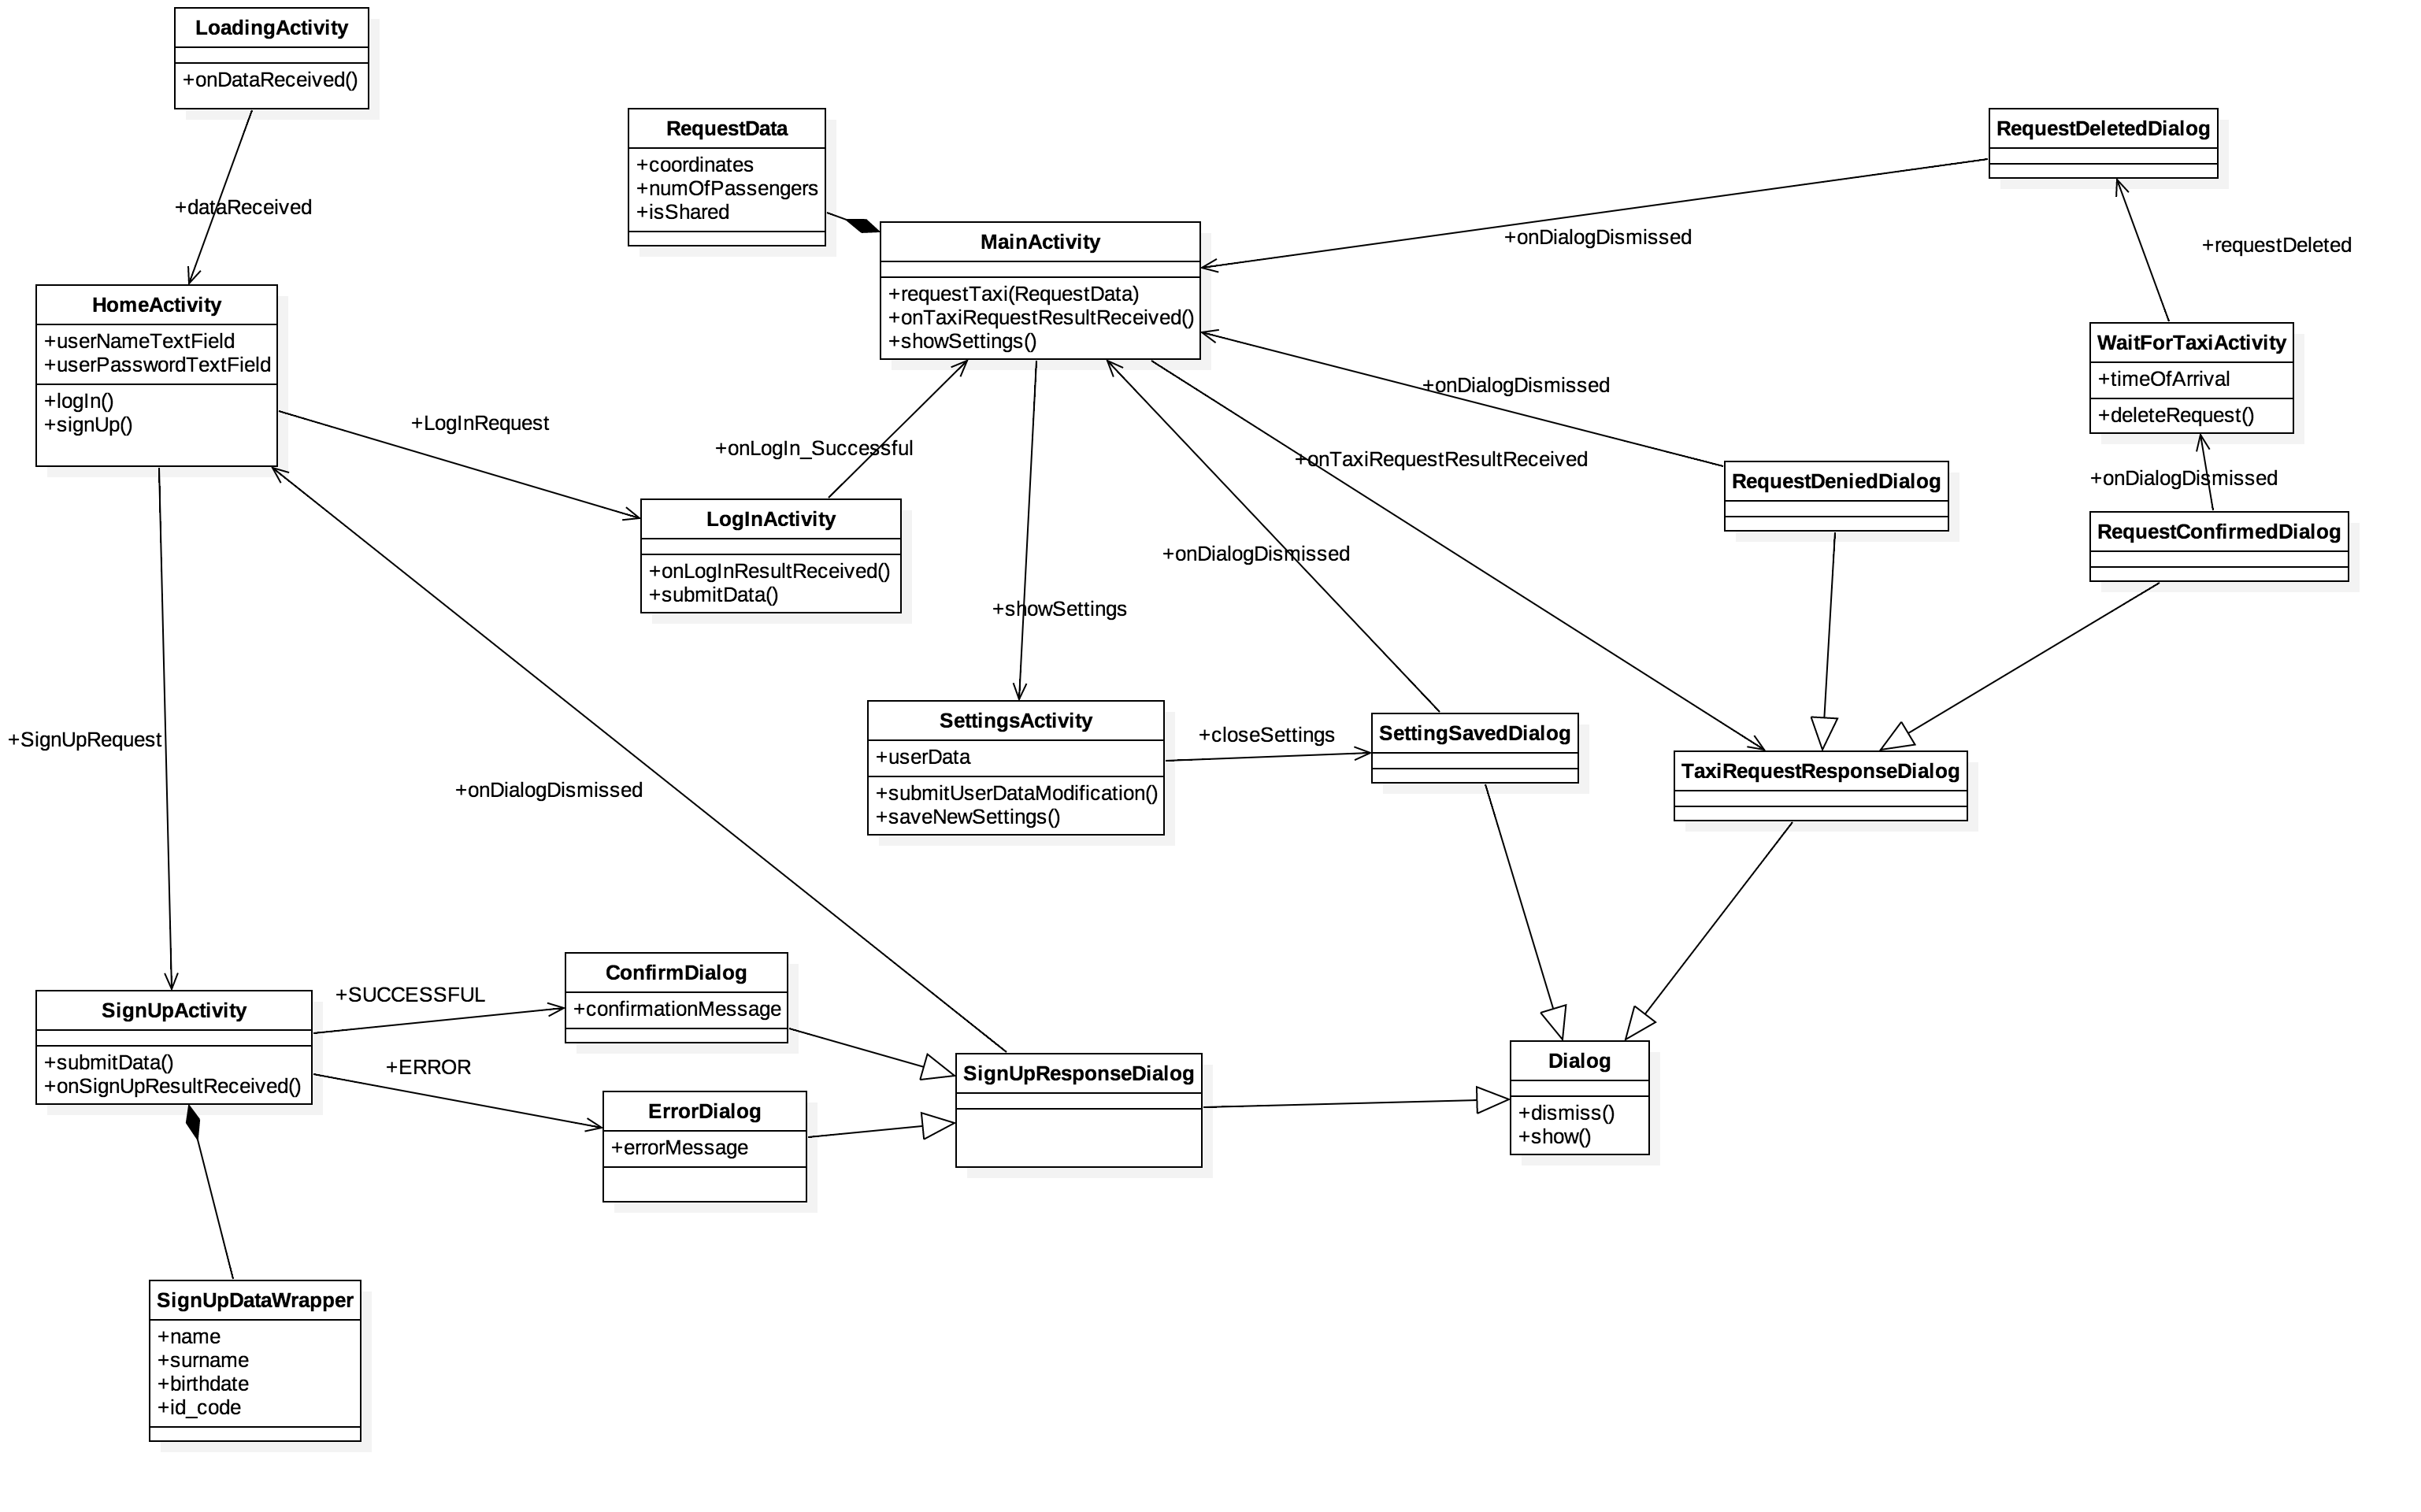
\includegraphics[width=\textwidth]{diagram/png/userAppClass}
\centering
\end{figure}
\vfill
\clearpage


\newpage
\vfill
\begin{figure}[h!t]
\caption{Driver Class Diagram}
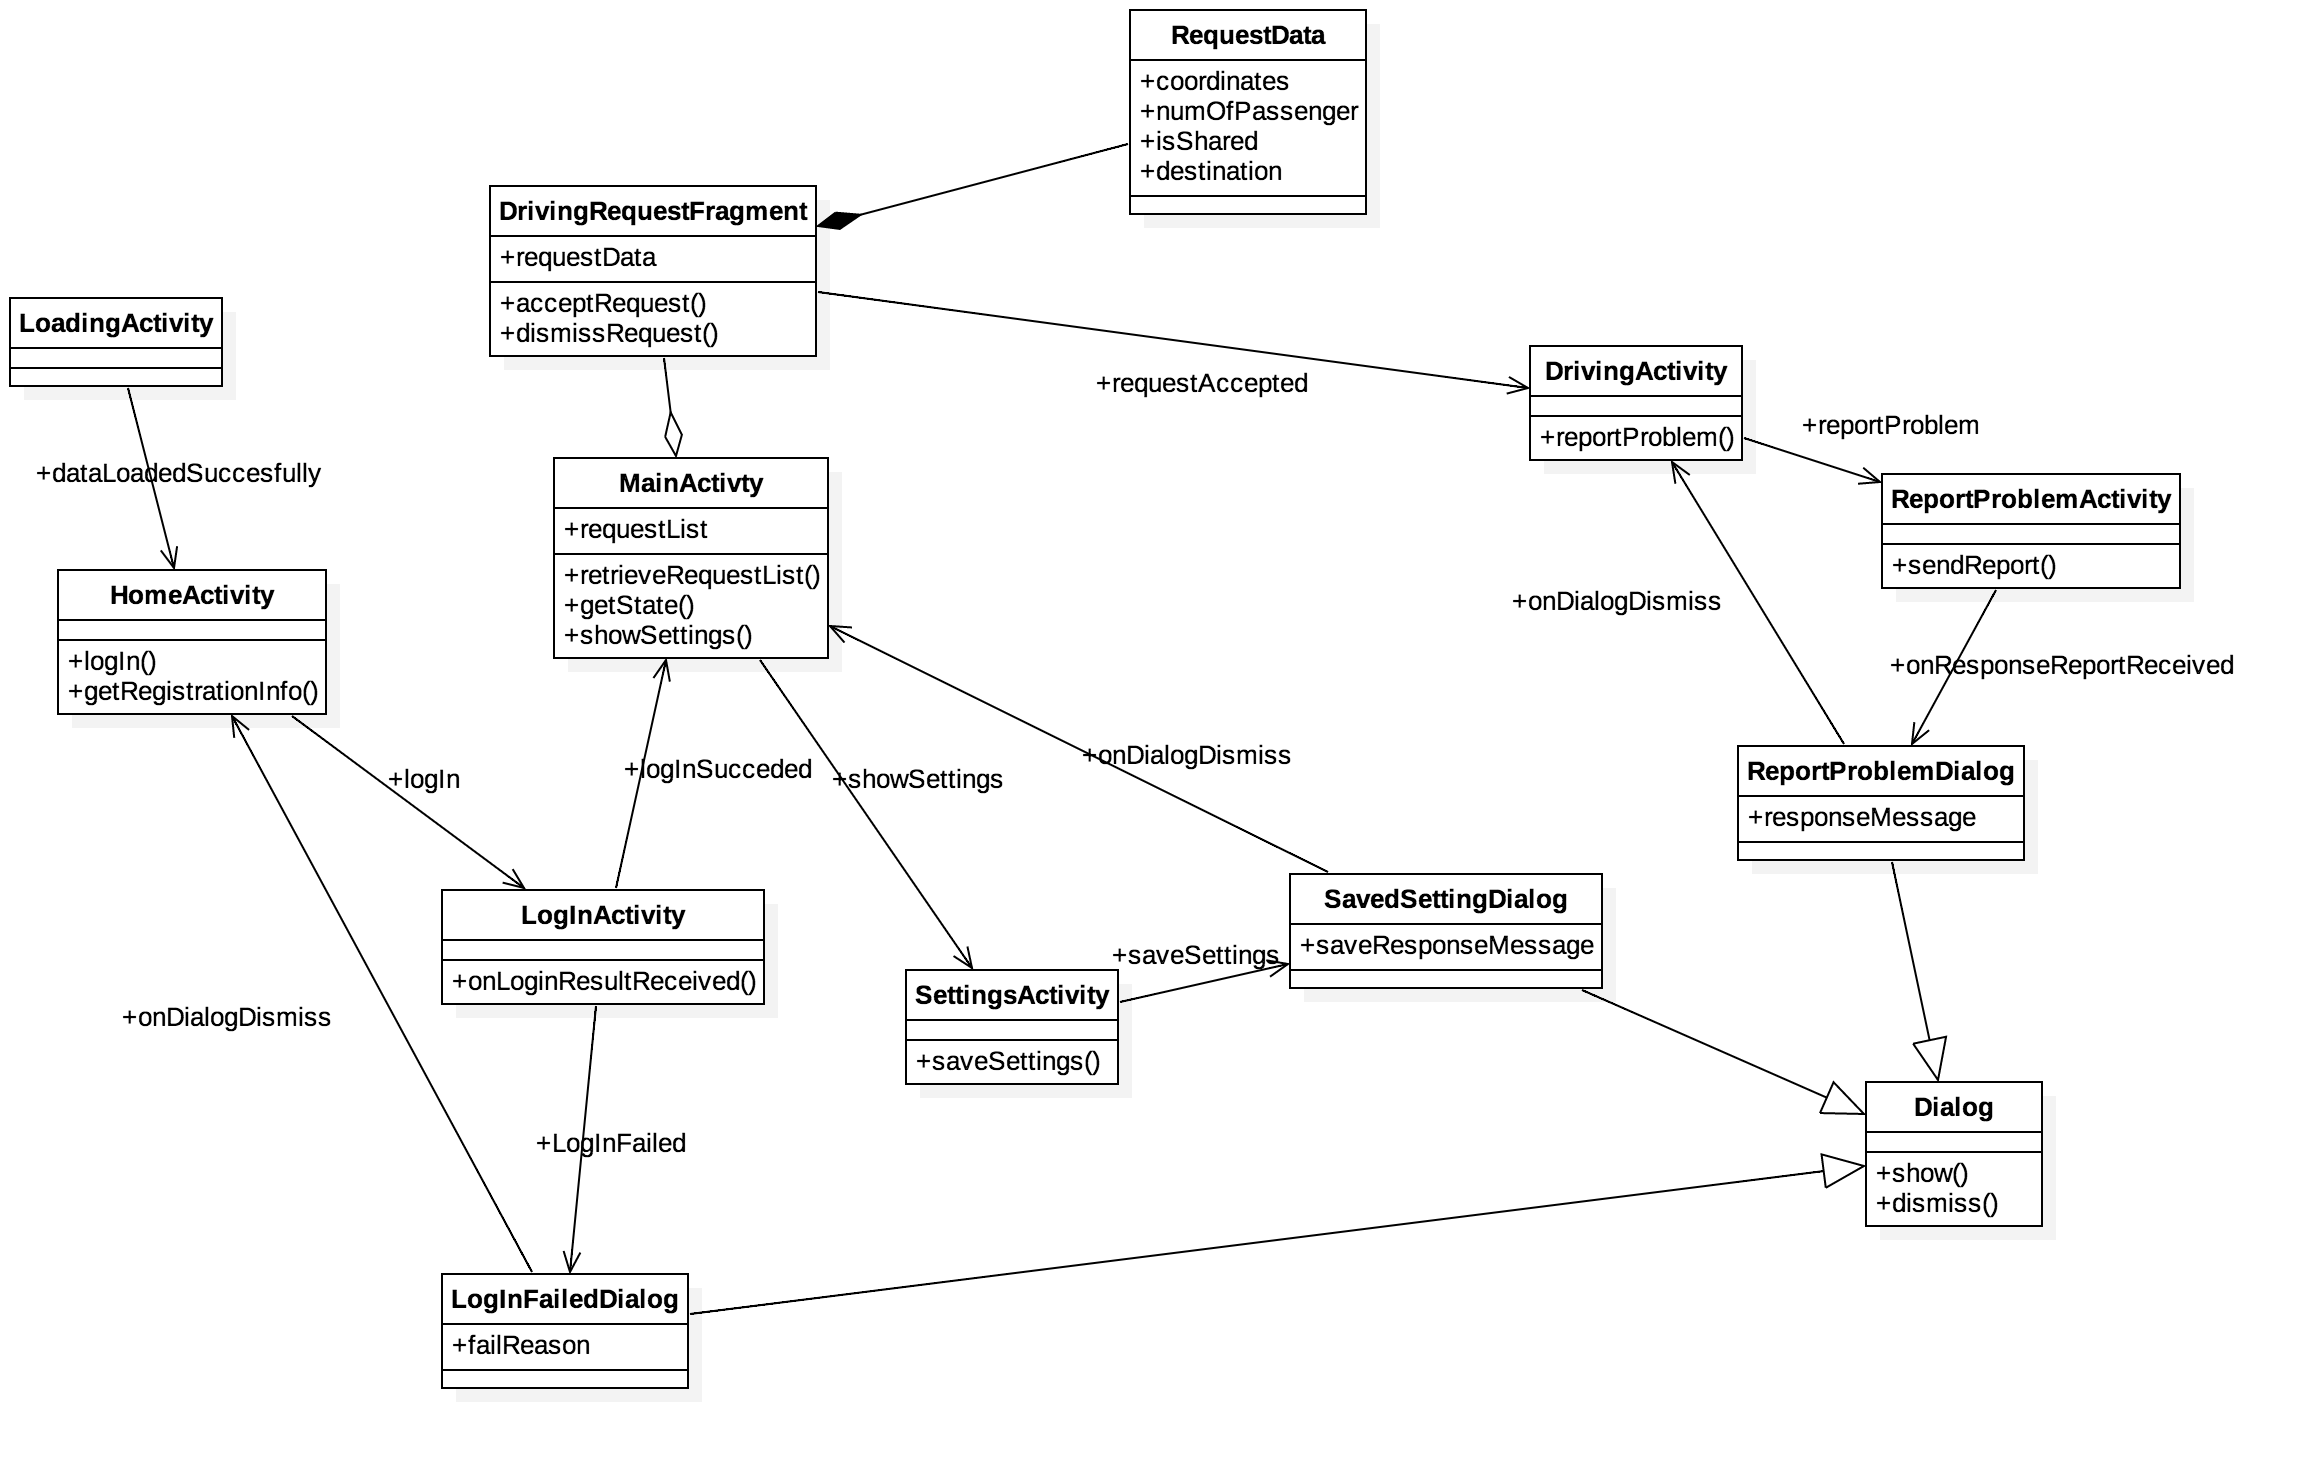
\includegraphics[width=\textwidth]{diagram/png/driverAppClass}
\centering
\end{figure}
\vfill
\clearpage






% section component_view (end)
